% !TEX root = ../main.tex

\chapter{绪论}

\section{研究背景与意义}


1.编排在开发中的地位
2.编排的作用是什么
3.自动化编排的意义
4.LLM赋能自动化编排




近年来,人工智能在经济发展和社会治理中展现了广泛的应用潜力。《中华人民共和国国民经济和社会发展第十四个五年规划和2035年远景目标纲要》明确提出,未来十年内,人工智能将在关键核心技术方面取得重大突破,推动智能化在各个领域的应用。“十四五”期间提出的三大人工智能发展布局——突破核心技术、打造数字经济新优势、营造良好数字生态——为多个行业的智能化升级奠定了坚实的基础。随着大语言模型(Large Language Model, LLM)的快速发展,其在智能系统构建中的应用价值愈发显著。通过将LLM与不同领域的工具集成,能够有效提升用户体验和系统效率。例如,基于大语言模型的智能体可以调用多种相关API,自动识别用户需求,为用户提供灵活高效的解决方案。

在多工具协同的智能系统中,编排扮演着不可或缺的角色,其主要任务是将分散的工具、模块或服务按照任务目标进行组织和协调。编排的作用在于将复杂任务拆解为多个子任务,并通过工具之间的逻辑关系和数据流动完成整体任务。它不仅是实现多工具集成的关键技术,也是提高系统自动化和智能化水平的重要途径。通过编排,系统能够在单一工具功能的基础上实现更高层次的组合功能,同时确保各工具间的数据交互和逻辑调用的正确性。这种能力在现代智能系统中尤为重要,尤其是面对用户需求动态变化或任务逻辑复杂的场景,编排可以显著提升任务执行的效率和准确性。

传统的编排方式通常依赖于硬编码规则或人工设计的编排逻辑。开发者需要手动定义工具之间的调用顺序、参数传递方式以及依赖关系,这种方式具有显著的局限性。首先,学习门槛较高,编排逻辑的构建往往需要开发者具备丰富的领域知识和编程能力,这对系统的开发效率造成了限制。其次,人工编排通常需要耗费大量人力资源,尤其是在复杂任务场景中,开发和维护编排逻辑可能会成为系统开发的瓶颈。此外,传统编排方式缺乏灵活性,无法动态适应用户需求或环境变化。例如,当某些任务路径未事先定义或任务依赖出现新变更时,系统往往无法根据实时输入自动生成适应性路径。这些缺陷使得传统编排难以满足现代智能系统中多工具集成、实时响应和动态适配的需求。

随着自动化编排技术的兴起,系统的灵活性和效率得到了显著提升。自动化编排能够通过逻辑推理和动态规划的方式,根据任务需求自动生成工具调用路径,降低了对人工干预的依赖,同时提高了系统的适应性和可扩展性。通过引入大语言模型,自动化编排在理解复杂任务需求和动态生成逻辑路径方面进一步增强。大语言模型凭借其强大的语义理解和生成能力,可以在未明确定义路径的情况下,基于用户目标实时推断出合理的任务执行流程,显著提升编排系统的智能化程度。例如,在需要协调多工具的复杂任务中,大语言模型能够准确识别工具间的依赖关系,优化工具调用顺序,并根据环境变化动态调整任务规划。

在此过程中,知识图谱的角色也发生了显著转变。过去,知识图谱主要用于构建领域内的结构化知识,建立实体及其关系网络,帮助系统实现更加精准的信息检索和问答。它依赖专家手工构建或自动化系统提取的知识,能够为特定领域中的推理提供逻辑支持。知识图谱的强项在于关系推理、知识验证以及为复杂任务提供可解释性。而如今,在大语言模型的语境中,知识图谱不再仅仅是孤立的信息源,而成为大语言模型的重要补充和增强工具。大语言模型具备广泛的语义理解和生成能力,但由于缺乏严格的逻辑结构和推理框架,有时会出现逻辑不连贯或生成内容不够精准的问题。知识图谱可以弥补这一不足:通过将结构化的知识与大语言模型结合,知识图谱能够为大语言模型提供精准的背景信息与逻辑推理能力。具体而言,在智能系统工具调用中,知识图谱可以帮助大语言模型识别工具之间的关系,辅助调用路径的优化,并增强模型的可解释性和推理能力。

尽管大语言模型在工具调用和集成方面展现了显著的潜力,仍然存在以下关键问题:一是无法集成大规模工具。当前的系统虽然可以调用多种API,但面对大量的工具集成时,表现出局限性。大语言模型需要处理不同工具的数据格式、调用方式以及响应速度,当工具数量较大时,模型的调用能力和协调效率会明显下降,难以实现对大规模工具的无缝集成。这种限制影响了系统在复杂场景中的适应性与灵活性。二是难以处理工具之间的依赖关系。对于涉及多个工具协同工作的任务,模型在处理工具间的依赖关系时往往力不从心。例如,某些工具的输出需要成为下一个工具的输入,且各工具的调用顺序和逻辑关系十分重要。目前,大语言模型难以有效管理这些复杂的依赖关系,容易导致任务流程的中断或结果的误差。



\section{国内外研究现状}

本节将会概述针对大语言模型智能体工具调用与工具图谱的研究进展。
首先,本节会介绍大语言模型智能体工具调用方面的研究,包括不同的流程搭建和提示词工程的方法,详细介绍了各种提升模型在工具编排、调用方面的能力。
其次,本节还会介绍有关图谱与大语言模型结合的应用场景,特别是在工具图上的应用,比如通过对工具之间的时序关系、资源依赖关系建模,从而得到工具调用路径的现有方法。

\subsection{大语言模型智能体工具调用}

为大型语言模型(LLMs)引入外部工具显著增强了智能体在应对复杂现实任务时的能力\cite{huang2024planning, Qin2023, qu2024tool}。
通过支持功能调用,LLMs 能够获取最新信息、提升专业技能、
执行精确计算并调用第三方服务,同时功能调用也能提高回答生成过程中的透明性和鲁棒性,让回答更具有可解释性和可靠性。
因此大语言模型智能体在多个领域实现了广泛的应用,例如多媒体内容搜索\cite{Song2023}、财务分析\cite{theuma2024equipping}以及旅行规划\cite{hao2024large}。

然而,要充分发挥功能调用的潜力并高效完成复杂任务,必须应对功能调用本身所带来的技术挑战。这些挑战并不仅限于简单的接口调用,而是伴随着实际应用场景的多样化需求和复杂性。例如,从如何管理多种 API 的协作,到如何优化工具调用的顺序和数据依赖关系,这些都对大语言模型的能力提出了更高的要求\cite{huang2024planning, Qin2023}。为深入理解这些问题,我们需要分析功能调用在实际应用中的复杂性及其解决思路。

功能调用的复杂性主要来自实际应用中 API 的多样性、复杂性及其相互依赖的特性\cite{Qin2023}。例如,现实场景中的 API 参数往往不仅限于简单的字符串或数字,还可能包括列表、字典、嵌套结构,甚至这些类型的组合。参数的数量可以从零到几十不等,其应用领域覆盖了多个行业和业务场景\cite{ye2024tooleyes}。此外,为完成一项任务,通常需要多个工具协同工作,单一 API 难以满足复杂任务的需求\cite{huang2024planning}。更复杂的是,一个 API 的输入可能依赖于另一个 API 的输出\cite{Qin2023},进一步增加了功能调用的挑战性和复杂性。

在大语言模型工具调用上,可以通过微调和非微调的方式来提升大语言模型的工具调用能力。
\cite{Qin2023, schick2024toolformer, hao2024toolkengpt, parisi2022talm}等研究者通过微调开源的大语言模型来增强模型的工具能力。然而这些方法通常需要额外的工具调用数据集来进行参数微调,
难以扩展到闭源的黑盒LLMs。并且该方法在以“即插即用”方式集成外部工具方面缺乏灵活性。
因此,本方案不涉及到对大语言模型的微调,我们仅介绍不需要参数微调的实现方式。

大语言模型的工具调用流程通常可以划分为以下四个核心阶段\cite{Ruan2023, Shen2023, Song2023}:任务规划、工具选择、工具调用和响应生成。尽管其他框架可能存在差异,但通常也是在此基础上进行修改、合并或删减。接下来,我们将按照这些模块化分层依次展开介绍。

\subsubsection{工具任务规划}

在现实的信息查询场景中,用户的查询需求往往包含复杂的意图,如何识别用户意图并明确定义好任务是工具调用的首要问题。
因此在工具任务规划阶段,我们首先需要将用户的需求语句转化为更加明确的任务,并对复杂任务进行拆解。

现有研究\cite{Miao2023}表示,大语言模型能够通过少样本甚至零样本实现有效的任务规划。
HuggingGPT\cite{Shen2023}首先把任务分解为各种子任务,然后选择合适的模型来解决这些子任务。
RestGPT\cite{Song2023}引入了一种从粗粒度到细粒度的规划方法,能够指导大语言模型逐步对任务进行分解。

\subsubsection{工具选择}

在任务规划阶段完成后,需要根据每个子任务进行工具选择。工具选择过程一般有两种途径:一种是通过训练得到的检索器来选择工具,另一种是直接让大语言模型从工具列表中选择合适的工具。

基于检索器的工具选择:当工具数量过多时,通常会使用检索器先搜索得到与任务相关的工具。检索方式包括基于关键词的检索和基于语义的检索两种。
基于关键词的检索:通过精确匹配实现用户需求和文档之间的对齐和查询,如TF-IDF\cite{Jones1972}和BM25\cite{Robertson2009};
基于语义的检索:利用神经网络来学习文本之间的语义关系,然后使用余弦相似度等算法计算语义相似度,如ToolLLM\cite{Qin2023},在其中作者们对BERT模型在工具数据集上进行微调,
提升了其在工具检索场景上的能力,进一步增强了基于语义检索的准确性。

基于大语言模型的工具选择:在工具数量有限,或者是已经检索得到少量有关工具时,可以让大语言模型利用自身的推理和分析能力选择最合适的工具。
具体来说,我们可以将备选工具信息与用户需求一起放入大语言模型的输入上下文,提供给模型。随后,模型根据用户需求选择合适的工具。

通用的提示词技巧可以帮助在多个工具中选择正确的工具。Chain of Thought(CoT)\cite{Wang2023a}在提示词中加入了例子,让大模型在解决复杂问题时采取相应的推理步骤,让大模型以分步的方式来规划和行动。Re-Prompting\cite{Raman2022}在生成计划之前会检查每个步骤是否能够执行。如果不能够执行,则让大模型重新生成计划。Self-consistent CoT(CoT-SC)\cite{wang2022self}因此让大模型执行多条推理路径,选择出现频率最高的答案输出。Tree of Thoughts(ToT)\cite{Yao2023a}用树状的形式组织推理过程,树上的每个节点表示一个“想法”即推理中间步骤。中间步骤的选择基于大模型的评估,最终计划用深度优先遍历(DFS)或者广度优先遍历(BFS)得出。在GoT\cite{Besta2023}中,作者把用树状结构组织推理扩展为了用图结构组织。
引入环境反馈同样可以提升能力,ReAct\cite{Yao2023b}中指导大模型按照指定格式来思考和行动。生成的想法来帮助大模型进行推理和规划,基于这个想法大模型会采取不同的行动,最后观察该行为的结果并作为反馈提供给大模型。Voyager\cite{Wang2023b}里智能体接收的反馈包括三种:程序执行的中间结果、执行错误描述和自我验证结果。Inner Monologue\cite{Huang2022}主动获取人类的反馈,将其与环境反馈进行结合,用于增强大模型的规划和推理能力。SelfCheck\cite{Miao2023}则让智能体对自己的推理步骤进行检查和评估,根据结果来修改计划以提升性能。

关于专门针对工具选择场景的提示词工程和流程搭建工作,ToolNet\cite{Liu2024}将大量工具组织成为有向图的形式,允许大语言模型从初始节点出发,迭代地在图上选择下一个工具,直到走到标记为结束节点的节点。
ToolLLM\cite{Qin2023}中提出了基于深度优先遍历算法的决策树算法,通过支持回溯操作解决了在工具选择上的错误传播问题,有效提高了整体的准确性和通过率。
AnyTool\cite{Du2024}提出了一种自我反思的层次化选择的方法,通过在结构化的工具调用树上迭代选择合适的工具。

在真实场景中,工具的数量通常非常庞大。如果将所有工具的描述都作为 LLM 的输入,会面临上下文窗口长度限制和模型生成时间延迟的限制。
因此,近期的研究越来越多地关注先通过检索器筛选工具\cite{Qin2023, anantha2023protip, Liu2024} ,再让大语言模型进行选择。

\subsubsection{工具调用}

在工具调用部分,大语言模型主要负责根据工具描述文件来提取工具调用所需的参数,并对工具服务器请求服务。
这一过程要求 LLMs 不仅能够正确提取参数的内容和格式,还必须严格遵循规定的参数输出来输出。

无需微调的方法主要通过提示词工程、多智能体协作来提升工具调用能力。基于提示词工程的方法利用少样本(few-shot)技术提供参数提取的示例,从而增强 LLM 提取参数的能力\cite{Song2023, Liu2023a, Liu2024, hsieh2023tool}。
Reverse Chain\cite{zhang2023reverse}采用逆向思维,首先为任务选择最终工具,然后让 LLM 填写所需的参数;如果缺少参数,则基于描述选择额外的工具来补全参数,最终完成任务。
EasyTool\cite{yuan2024easytool}通过提示 ChatGPT 重写工具描述,使其更简洁并直接包含工具功能的使用指南,增强 LLM 对工具功能和参数需求的理解。
ConAgent\cite{shi2024learning}引入了一种多智能体协作框架,其中一个专门的执行智能体负责任务执行和工具调用。

\subsubsection{响应生成}

由于工具输出形式多样且复杂,这些结果可能以文本、数字、代码等不同格式呈现,因此无法直接提供给用户查看。需要通过大语言模型(LLM)对这些输出进行组织和分析,围绕用户的查询提取相关信息,并结合模型自身的知识生成完整且清晰的回答。根据将工具输出融入大语言模型提示词的方式,现有方法主要分为直接插入方法和信息整合方法两类。

直接插入方法是早期研究中常见的一种实现方式 \cite{schick2024toolformer, wang2024tools, hao2024toolkengpt}。
模型会首先输出带有占位符的回答,在得到工具调用结果后将占位符替换为工具结果。
然而,由于工具输出结果的形式和内容往往难以预测,这种方法可能会影响用户体验。

为了克服这一问题,许多研究选择将工具输出作为上下文的一部分输入到 LLM,以便生成更高质量的响应 \cite{shen2024hugginggpt,}。
不过,由于 LLM 的上下文长度有限,对于某些工具输出内容,直接输入会面临挑战。
为此,不同方法提出了多种解决方案。例如,RestGPT \cite{Song2023} 通过预定义模式(schema)来简化冗长的工具输出,这些模式包括示例、格式和可能错误的说明文档。
ToolLLaMA \cite{Qin2023} 采用截断策略,将输出裁剪到适当的长度范围内,但可能因此丢失解决用户问题的关键信息。
ReCOMP \cite{xu2023recomp} 提出了一种压缩机制,可以将冗长的工具输出浓缩为简洁的版本,仅保留核心内容。

\subsection{大语言模型与工具图谱结合的应用}

尽管大语言模型主要用于纯文本的场景,但是在许多现实场景中,文本数据与丰富的结构信息以图谱的方式存储。
此外,大语言模型的基于文本的推理能力已经得到较多的展现,但是大语言模型在图谱上的推理能力仍有很大的探索空间。

通过将现实世界的知识表示为结构化的知识图谱,并在图谱上进行推理和演算,能够解决许多重要问题。

关于如何将图谱上的知识提供给大语言模型的问题,有三种常见的方法:

自然语言描述。用自然语言描述图结构是最简单的方式,可以直接描述图上的边和邻接列表;对图进行文本上的改写。由于自然语言描述图通常会较为复杂,而且不具备结构化的特点,因此对图的描述进行了改写,得到了更加高效的图的描述,有利于模型对图谱信息的利用;对图进行编码。最后一种方法是通过训练图编码器,将图结构编码成为特征序列并作为特征的一部分输入到大语言模型中。这种方法涉及到对大语言模型的微调,以让其适应新的输入格式。

通过将图谱的信息通过自然语言文本或者嵌入向量的格式输入到大语言模型上,可以在图谱上进行推理和搜索。
常见的做法是利用深度优先搜索算法(DFS)或者广度优先搜索算法(BFS)来实现在图上的推理和搜索。
许多研究探索了基于搜索的推理,特别是在知识图谱领域。
Reasoning on Graph\cite{Luo2023}的方法将知识图谱作为可靠的知识来源,通过提示大语言模型生成多个关系路径作为计划,
随后根据这些路径不断在知识图谱上搜索,有效地提高了回答的可信度和效率。
另一种方法是在图谱上动态地进行迭代检索和推理子图来模拟动态搜索过程\cite{Liu2024, Sun2023, Ma2024}。在每个步骤中,大语言模型都检索当前节点的邻居节点,然后决定下一步操作是继续搜索还是结束搜索并给出答案。
在ToolNet\cite{Liu2024}中,作者根据工具调用的数据集建立了图谱,并根据图谱上的边进行搜索,迭代式选择所需的工具进行调用,有效提升了工具搜索的准确性。
Think-on-Graph系列\cite{Sun2023,Ma2024}在知识图谱上通过大语言模型Agent进行迭代式的束搜索,探索发现最好的推理路径,并返回最有可能的推理结果。
GNN4TaskPlan中\cite{wucan2024}通过构建工具图和使用图神经网络,实现了非训练和基于训练的两种方式,使用图神经网络与当前流行的提示词工程的方法形成了互补,能够有效提升大语言模型在任务规划上的准确性。
ControlLLM\cite{Liu2023a}引入了一种叫做“在图上思考”(Think-on-graph, ToG)的范式,通过深度优先搜索算法(DFS)在构建好的工具图上进行搜索,得到解决方案。

这些方法的优点在于,通过图谱的辅助,系统不仅能够提供对应的答案,还可以提供图谱片段作为可以解释的证据。同时,由于知识图谱存储的数据量可以扩展,这些方法通过在图上搜索也增加了系统的可扩展性。

\section{研究问题}

基于以上的研究背景,本文的核心研究问题归纳如下:
\begin{itemize}
    \item \textbf{如何通过工具调用路径数据构建一个高效且结构化的工具图谱?}
   本问题旨在研究如何筛选、清洗现有的工具调用路径数据,并构建一个大型工具图谱,从而将路径中的工具知识有效地嵌入到图谱中。重点探讨数据清洗的标准和方法、知识图谱构建的技术路径,以及如何使该图谱在后续的工具搜索和优化流程中发挥有效作用。
    \item \textbf{如何结合知识图谱与智能体架构实现自动化工具编排和调用?}
   本问题关注如何基于知识图谱和智能体架构,设计一个完整的任务分解、工具选择、调用以及结果解析的流程框架。研究重点包括:智能体如何高效利用知识图谱进行工具调用路径的优化,如何在真实API环境下验证智能体编排的有效性,以及如何提升工具调用的精确性和任务完成效率。
\end{itemize}

\section{研究内容}
本文主要研究基于Agent与图谱的任务编排工具的设计与实现流程,主要针对用户进行信息查询时的便利。本文研究与实现的内容主要包括以下几点:

\begin{enumerate}
    \item 本文提出了一种基于工具调用路径数据构建大型工具图谱的方法,旨在辅助智能工具搜索与调用流程。首先,通过两种数据筛选策略,筛选出高质量的API工具调用路径数据。接着,设计了工具点权和边权值的计算方法和动态更新方法,以表示工具之间的转换关系和工具可用性。最后,通过对比包含图谱知识与传统检索增强方式,验证了工具图谱在实际应用中的有效性。
    \item 为了有效利用构建的工具图谱的知识,本文提出了基于DFS的工具动态搜索算法。该方法通过在图谱上进行深度优先搜索和动态回溯,能够充分利用图谱上的知识选择工具路径。同时,我们提出了记忆框架,通过维护记忆知识,进一步辅助大语言模型的规划和推理。通过在真实世界的API测试集上进行实验,验证了该方法的有效性,并且证明该方法优于基线方法。
    \item 本文设计并实现了一个基于知识图谱和大语言模型的智能API编排与调用系统,旨在提供用户友好的交互体验。本工作允许用户通过自然语言提问,系统能够解析需求并自动调用相关API,生成答案。其主要功能包括用户登录、API调用流程可视化、问答服务以及自定义工具添加,而管理员可以管理模型超参数配置和数据库。系统的整体架构分为存储层、访问层、功能层、接口层和展示层五层,各层负责不同的功能,以确保系统的高效性和易用性。
\end{enumerate}

\section{论文组织结构}

如图\ref{fig:ch1-structure}所示,本论文的内容组织结构分为以下几章:

\begin{figure}[!htp]
    \vspace{1em}
    \centering
    \setlength{\abovecaptionskip}{10pt} % 控制图片和caption之间的距离
    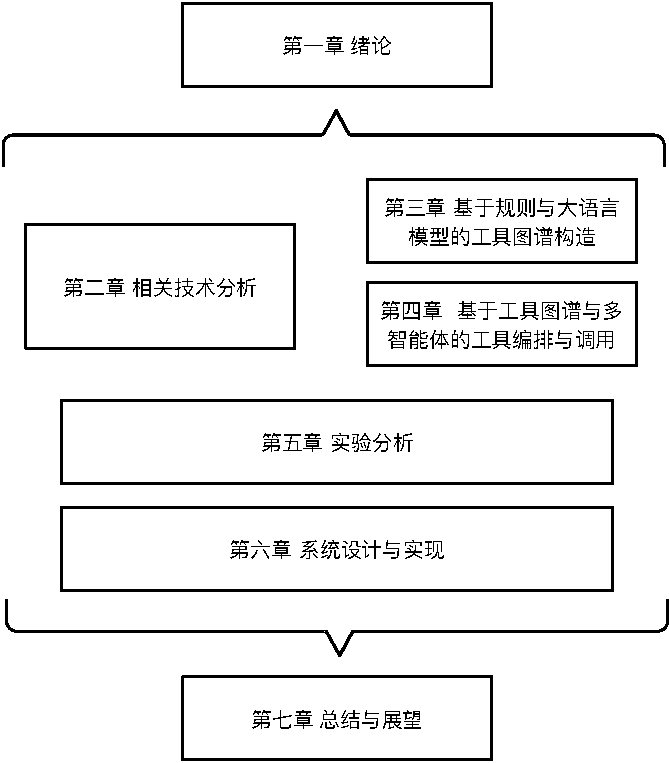
\includegraphics[height=9cm]{../assets/ch1-论文结构.pdf}
    \bicaption{论文组织结构}{Structure of the Paper}
    \label{fig:ch1-structure}
  \end{figure}

  \indent 第一章为绪论,本章从研究背景出发,简要阐述了研究的问题与难点,分析了国内外的研究现状,介绍了本文的主要工作内容,并对全文的组织结构进行了概述。

  \indent 第二章为相关理论与技术,本章主要介绍了研究相关的核心概念与技术背景。首先,介绍了知识图谱的定义、分类及基于API的知识图谱研究;其次,阐述了大语言模型的定义、发展历程及其关键技术,包括大模型智能体、提示词工程和检索增强技术等;最后,探讨了大语言模型与图谱结合的应用方案及其典型案例。
  
  \indent 第三章为基于工具调用路径的工具图谱构建方法及实现,本章提出了一种利用工具调用路径数据构建大型工具图谱的方法。内容包括数据筛选与清洗、图谱结构的设计,以及通过边权和点权更新工具间关联的方法,为后续工具搜索流程提供支持。
  
  \indent 第四章为基于知识图谱和智能体的工具编排和调用方法的设计与实现,本章聚焦于基于大语言模型智能体的工具任务解决方案,涵盖任务分解、工具选择、工具调用及结果解析等关键流程,并探讨了知识图谱在工具任务编排中的核心作用。
  
  \indent 第五章为实验分析,本章通过对API检索器模型进行实验,验证了微调模型在工具检索中召回率和NDCG指标的提升。随后,对整体的API编排与调用流程进行了评估,结果与多个基线方法进行对比,证明了本文方法的可行性与优越性。此外,通过消融实验,进一步验证了系统中各模块的必要性及贡献。
  
  \indent 第六章为系统设计和实现,本章在前几章的基础上完成了系统的架构设计和功能模块实现,最终构建了可视化界面及任务流程平台。具体内容包括系统框架设计、关键功能模块开发及系统展示。
  
  \indent 第七章为总结与展望,本章回顾了全文的研究工作,概括了主要成果,并针对本研究的局限性提出改进方向,展望了未来在知识图谱与大语言模型结合领域的研究前景。